% Author normalized to 'Jaron Mar' for repo consistency (CITATION.cff/LICENSE).
% Figure paths rewritten from Claude Science artifact markers to local figs_c2c/.
\documentclass[11pt]{article}
% ==================================================================
% JUDGE CUT — condensed companion to the full technical manuscript
% "From Clocks to Coordinates" (manuscript_bodyvector.pdf, 53 pp).
% Leads with the perturbation discovery. Every number is lifted verbatim
% from the frozen artifacts cited in the full manuscript; nothing new is asserted.
% ==================================================================
\usepackage[utf8]{inputenc}
\usepackage[T1]{fontenc}
\usepackage[margin=0.9in]{geometry}
\usepackage{amsmath,amssymb}
\usepackage{graphicx}
\usepackage{booktabs}
\usepackage{siunitx}
\usepackage{authblk}
\usepackage{xcolor}
\usepackage[hidelinks]{hyperref}
\hypersetup{
  pdftitle={From Clocks to Coordinates (judge cut)},
  pdfauthor={Jaron Mar}
}
\usepackage[numbers,sort&compress]{natbib}
\usepackage{caption}
\captionsetup{font=small,labelfont=bf}
\sisetup{detect-weight=true,detect-family=true}
\newcommand{\D}{\ensuremath{D}}
\newcommand{\A}{\ensuremath{A}}
\newcommand{\wikr}{\ensuremath{\mathbf{w}_{I_{\text{Kr}}}}}
\newcommand{\Ikr}{\ensuremath{I_{\text{Kr}}}}

\title{\textbf{From Clocks to Coordinates:}\\
\textbf{Controlled Human Perturbations Reveal Hidden Directions in ECG Biological Age}\\[4pt]
\large\normalfont A condensed account of the central result}
\author[1]{Jaron Mar}
\affil[1]{University of Miami \quad \texttt{jim4226@miami.edu}}
\date{}

\begin{document}
\maketitle
\vspace{-2em}

\begin{abstract}
\noindent
Neural ``ECG age'' and organ-age models return a single scalar, collapsing biophysically
distinct processes into one number. This work shows biological age is better read as a
\emph{direction} in a state space. Four phase-of-heartbeat age clocks compress into a
\emph{shared axis} \A\ and an orthogonal \emph{disagreement radius} \D, with the geometry frozen
on CODE-15 \emph{before any outcome was read}. The radius \D\ was null on its single
pre-registered confirmatory mortality test (hazard ratio \num{1.01} per SD, 95\% CI
\numrange{0.98}{1.04}, $p=\num{0.48}$)---the honest negative that motivates a signed analysis.
A randomized \Ikr\ blocker (dofetilide) displaced the ST-T repolarization clock
($+\num{4.2}$~SD$\cdot$h, false-discovery-rate $p=\num{0.002}$), defining a covariance-scaled
signed \emph{direction} \wikr---the coordinate the unsigned radius discards. It was confirmed by
a second \Ikr\ blocker (quinidine, $+\num{0.83}$) and was specific relative to non-\Ikr\
comparators; direction-derivation is exploratory (Holm-adjusted permutation $p=\num{0.069}$).
Frozen and carried into an independent external cohort (Chapman--Shaoxing/Ningbo,
$n=\num{44550}$, \num{386} QT-extension cases), it added \emph{conditional} information about
physician-assigned QT-interval extension beyond conventional intervals, \A\ and \D\ (fully
adjusted odds ratio \num{1.23} per SD, $p=\num{1.9e-4}$; marginally null---a suppression effect).
The shared axis \A\ was separately mortality-associated and generalized across the body. This
condensed account presents that result; a \num{53}-page technical manuscript provides the full
methods, the multiscale atlas (whole-body CT, brain MRI, an \emph{in-silico} genomic screen), and
every frozen artifact.
\end{abstract}

\section{The claim}
Biological-age models---whether a neural network reading an electrocardiogram or a volumetric
organ clock---almost always return \emph{one number}: an age gap. That scalar discards direction.
Two people equally ``old for their age'' may be old in physiologically opposite ways. The
question this work answers is whether that lost direction is real, measurable and
\emph{transportable}: can a controlled human perturbation reveal a fixed coordinate in an
age--state space, and does that coordinate carry information in a cohort that never saw the
perturbation?

\begin{figure}[t]
\centering
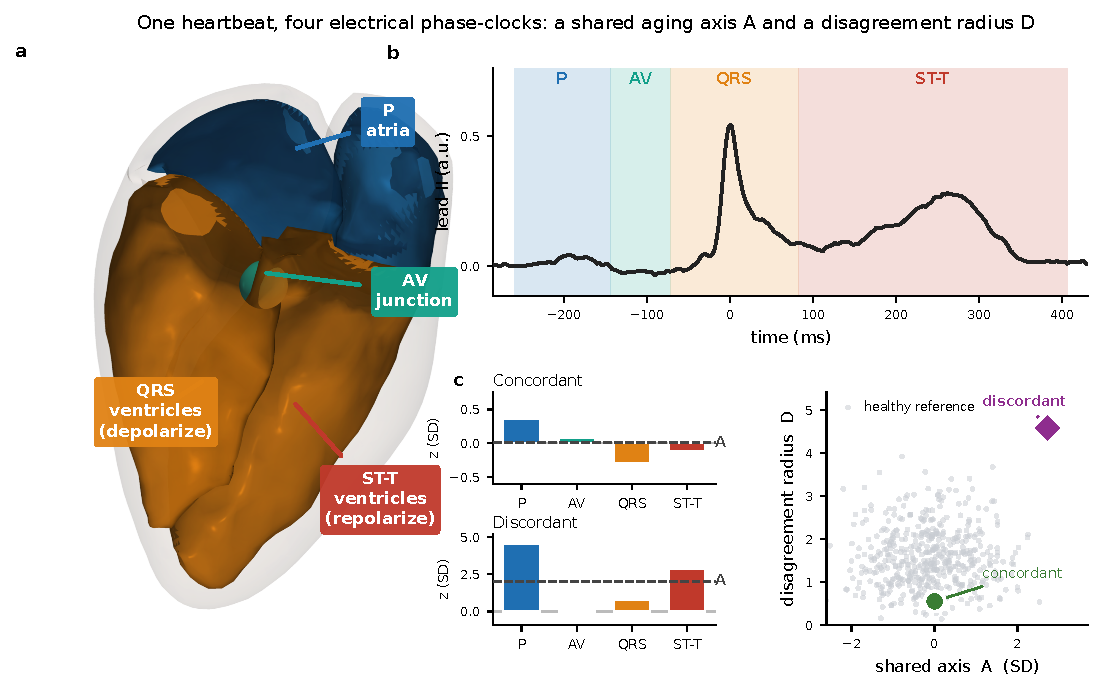
\includegraphics[width=0.96\linewidth]{figs_c2c/fig1_concept.pdf}
\caption{\textbf{Biological age as a vector, not a scalar.} Four phase-of-heartbeat age clocks
(P, AV, QRS, ST-T) are standardized against a frozen healthy calibration cohort and read as a
point in a four-dimensional gap space. Its coordinates are a \emph{shared axis} \A\ (the common
displacement---how uniformly old the heartbeat looks) and an orthogonal \emph{disagreement
radius} \D\ (how much the four clocks disagree). The geometry was frozen on CODE-15
(\num{233770}~patients) before any outcome was read.}
\label{fig:concept}
\end{figure}

\section{A shared axis that behaves like aging, and a radius that does not}
The shared axis \A\ behaves the way a biological-age summary should. In frozen CODE-15
development it was associated with mortality (hazard ratio \num{1.22} per SD); it generalized to
whole-body organ-system aging in NHANES ($+\num{1.21}$ per SD, 95\% CI \numrange{1.13}{1.29}) and
transferred geographically to a Chinese cohort ($r=\num{0.65}$; Fig.~\ref{fig:arobust}).

The disagreement radius \D\ was the original hypothesis: that \emph{how} the clocks disagree adds
prognostic information beyond the shared level. It does not. On its single pre-registered
confirmatory test---a model-frozen Cox likelihood-ratio test on the locked CODE-15 final-test
partition---\D\ was null (hazard ratio \num{1.01} per SD, 95\% CI \numrange{0.98}{1.04},
$p=\num{0.48}$; $n=\num{74715}$, \num{2583}~deaths). It showed no detectable association with
independent cardiac structure and did not change under acute physiological stress
(Fig.~\ref{fig:ddissoc}). Reporting that null honestly is what motivates the rest of the paper:
the \emph{unsigned} radius throws away a sign, and the sign is where the mechanism lives.

\begin{figure}[t]
\centering
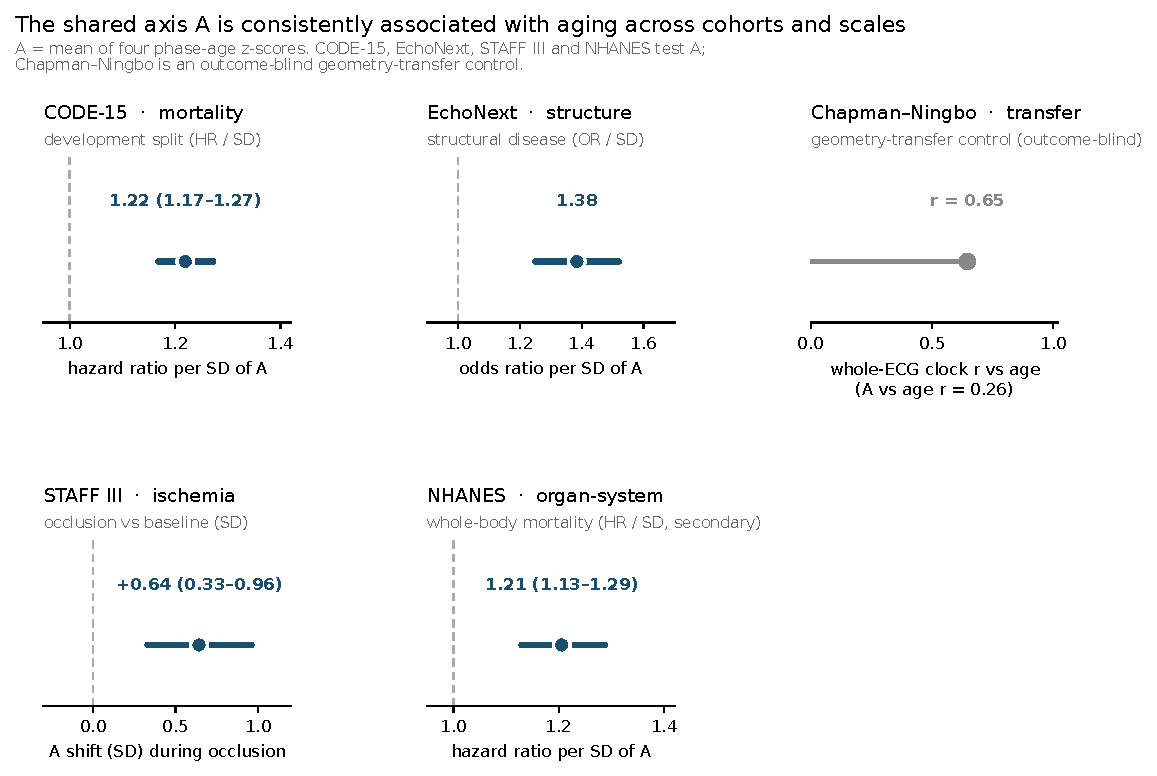
\includegraphics[width=0.82\linewidth]{figs_c2c/fig2_A_robust.pdf}
\caption{\textbf{The shared axis \A\ is consistently associated with aging across cohorts and
scales.} Development mortality, external geographic transfer, and whole-body organ-system aging
(NHANES) all point the same way. \A\ is the part of the decomposition that behaves like a
conventional biological-age summary.}
\label{fig:arobust}
\end{figure}

\begin{figure}[t]
\centering
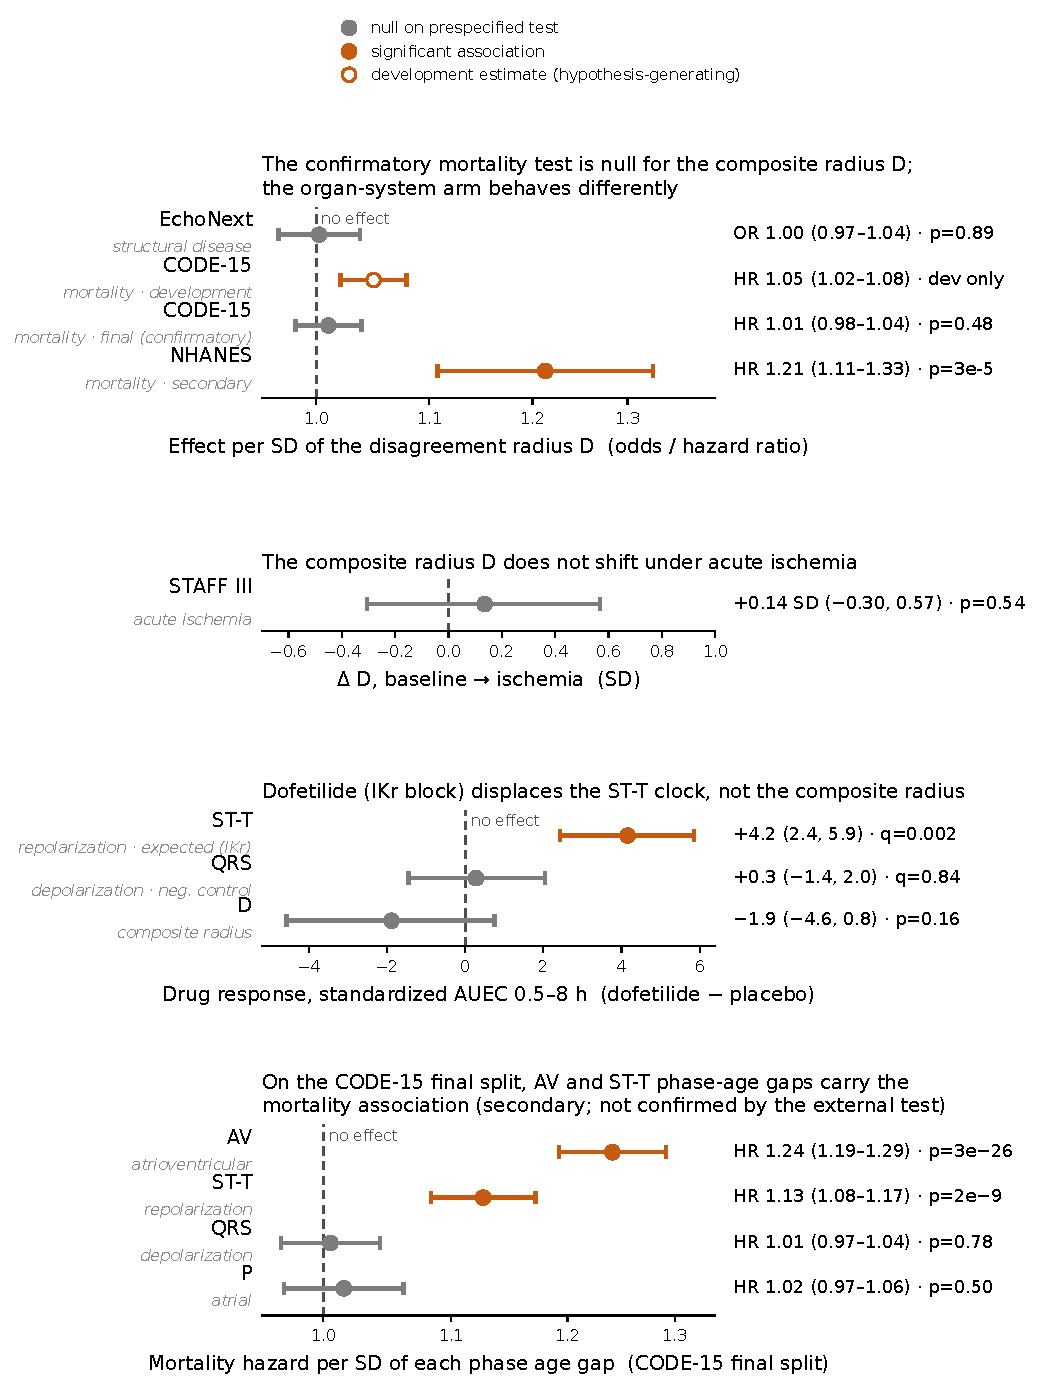
\includegraphics[width=0.82\linewidth]{figs_c2c/fig3_D_dissociated.pdf}
\caption{\textbf{The unsigned radius \D\ shows no detectable association with structure or
response to acute stress, and is null on its confirmatory mortality test.} The original radial
hypothesis fails. The signed coordinate that the radius discards, however, is not empty---it is
the subject of Fig.~\ref{fig:compass}.}
\label{fig:ddissoc}
\end{figure}

\section{A controlled human perturbation reveals a hidden direction}
The decisive experiment is a randomized-controlled human ion-channel perturbation. In the
ECG-RDVQ crossover study, a specific \Ikr\ (rapid delayed-rectifier potassium current) blocker,
dofetilide, was administered against placebo. \Ikr\ blockade has a textbook electrophysiological
signature: it prolongs repolarization, that is, the ST-T segment. If the age--state space is
physically meaningful, this perturbation should displace the ST-T phase clock along a
\emph{reproducible direction}.

It does. Dofetilide displaced the ST-T repolarization clock by $+\num{4.2}$~SD$\cdot$h
(false-discovery-rate $p=\num{0.002}$), while a negative-control QRS contrast was null. From the
mean placebo-corrected displacement $\mathbf{m}$, a covariance-scaled signed direction was
defined,
\[
\wikr=\Sigma_q^{-1}\mathbf{m}\big/\sqrt{\mathbf{m}^{\top}\Sigma_q^{-1}\mathbf{m}},
\]
precisely the coordinate the unsigned radius \D\ discards. Two independent checks make it more
than a within-study artifact. A \emph{second}, chemically distinct \Ikr\ blocker (quinidine)
projected positively on the frozen axis ($+\num{0.83}$, 95\% CI \numrange{0.52}{1.20}), a
held-mechanism confirmation. And the direction was specific: non-\Ikr\ comparators (ranolazine,
verapamil) had projections whose confidence intervals include zero (Fig.~\ref{fig:compass}b).
Because two perturbation directions (\Ikr\ and acute ischemia) were screened, the honest
multiplicity-corrected permutation test on the direction's magnitude is only nominal
(Holm-adjusted $p=\num{0.069}$); the direction-\emph{derivation} is therefore reported as
exploratory, and its confirmation comes from the external cohort below.

\begin{figure}[t]
\centering
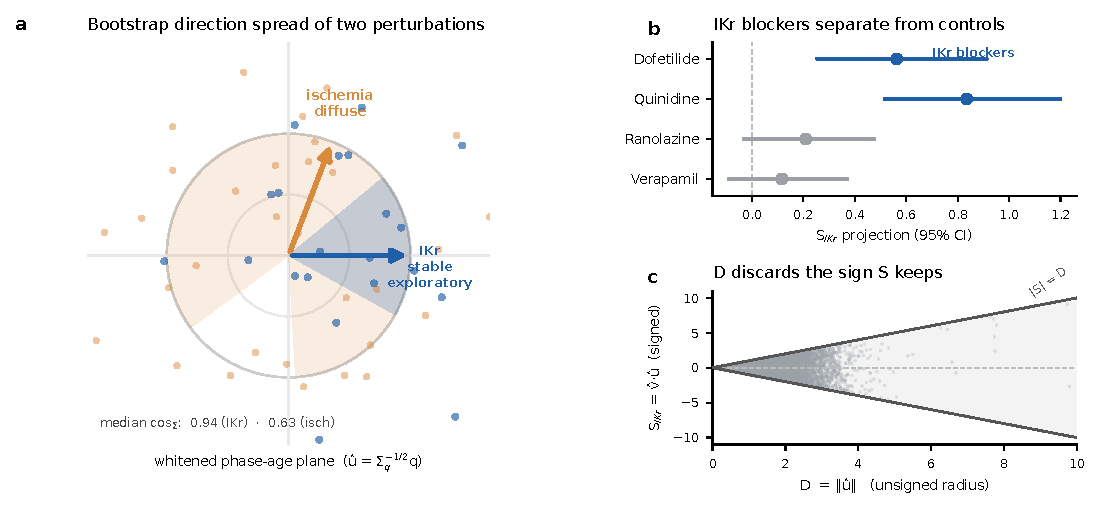
\includegraphics[width=0.9\linewidth]{figs_c2c/fig_perturbation_compass.pdf}
\caption{\textbf{An outcome-blind, signed perturbation direction recovers a mechanism the
unsigned radius discards, and is frozen for external transport.} \textbf{(a)}~Bootstrap spread of
the recovered direction in a two-dimensional slice of the three-dimensional whitened contrast
space: the \Ikr\ axis (blue) is tightly concentrated (bootstrap median $\cos_\Sigma=\num{0.94}$;
\num{9999} of \num{10000} bootstraps reproduce its sign with no alignment), whereas the
acute-ischemia axis (orange) is diffuse because ischemia moves the vector along the shared axis
\A\ rather than within the contrast subspace. \textbf{(b)}~The two \Ikr\ blockers separate from
zero; non-\Ikr\ comparators do not. \textbf{(c)}~In raw whitened coordinates the signed score is
bounded by the unsigned radius, $|S_{\text{raw}}|\le\D_{\text{raw}}$: the radius keeps the
magnitude and discards exactly the sign the perturbation axis recovers.}
\label{fig:compass}
\end{figure}

\section{The direction transports to an external cohort}
A direction is only useful if it carries information where it was never trained. The frozen \wikr\
was carried, unchanged, into an independent external cohort (Chapman--Shaoxing and Ningbo,
$n=\num{44550}$; \num{386} patients with a physician-assigned diagnosis of QT-interval extension
beyond conventional intervals). Added to a model already containing the shared axis \A, the
disagreement radius \D\ and the conventional intervals, the signed \Ikr\ score carried
\emph{conditional} information about that diagnosis (fully adjusted odds ratio \num{1.23} per SD,
95\% CI \numrange{1.10}{1.36}, $p=\num{1.9e-4}$; Firth-penalized odds ratio \num{1.22},
$p=\num{1.9e-4}$). The marginal association was null (odds ratio \num{1.00})---a genuine
suppression effect: the direction speaks only once the shared displacement and the conventional
intervals are held fixed, which is exactly what a hidden \emph{orthogonal} coordinate should do.
The per-site estimates agree (Ningbo odds ratio \num{1.20}, $p=\num{0.0019}$, \num{329}~cases;
Chapman--Shaoxing odds ratio \num{1.44}, labeled underpowered at \num{57}~cases).

\section{Why this is the result, and what the rest of the paper is}
The claim is narrow and falsifiable: a controlled human perturbation of a single ion current
defines a fixed, covariance-scaled direction in an ECG age--state space; that direction is the
signed coordinate an unsigned age-gap radius discards; and, frozen, it transports to an
independent cohort as conditional information about a clinically assigned repolarization
phenotype. The honest negative (\D\ is null on its confirmatory test) and the honest hedge
(direction-derivation is exploratory under multiplicity; the external cohort provides the
confirmation) are part of the result, not footnotes to it.

The full \num{53}-page manuscript carries the complete methods, the frozen-geometry protocol and
firewall, the acute-ischemia analysis (which moves \A, not a stable signed contrast, and explains
why ischemia fails the direction gate), and a deliberately \emph{supporting} multiscale
atlas---whole-body CT, brain MRI and an \emph{in-silico} genomic screen of Human Accelerated
Regions---that illustrates the same shared-axis/disagreement decomposition at other scales
without claiming to confirm the electrical result. Those arms are the visually rich companion
atlas; the perturbation direction above is the finding.

\begin{center}\itshape
Aging is not one number. It is a state space---and physiology moves through it in directions.
\end{center}

\end{document}
